\documentclass[11pt, letterpaper]{article}
\usepackage[utf8]{inputenc}
\usepackage{amsmath}
\usepackage{amssymb}
\usepackage{graphicx}
\usepackage{hyperref}
\usepackage{natbib}
\usepackage{geometry}
\usepackage{tikz}
\usetikzlibrary{positioning, arrows.meta, shapes.geometric, fit, backgrounds, calc}
\geometry{margin=1in}

\title{Addressing the Permissiveness Problem in Graph-Constrained Decoding with Dynamic Context-Aware Tries}
\author{Bernard \\
Department of Computer Science \\
University of Mines and Technology (UMaT)}
\date{\today}

\begin{document}

\maketitle

\begin{abstract}
    Large language models (LLMs) are powerful engines for multi-hop reasoning, yet their autoregressive architecture makes factual hallucination mathematically inevitable. Recent knowledge graph-constrained decoding frameworks, such as Graph-Constrained Reasoning (GCR), solve this by using precomputed prefix tries to restrict generation strictly to verifiable graph paths. However, this introduces a new limitation: the permissiveness problem. Because these static constraints rely entirely on graph structure and ignore question semantics, they admit thousands of valid but irrelevant reasoning paths, forcing the LLM to fall back on its hallucination-prone parametric memory to choose among them. To solve this, we introduce the Dynamic Context-Aware Trie (DCA-Trie), an upgraded constraint oracle that filters structurally valid paths using semantic relevance to both the question and the generated prefix. We also introduce the Semantic Irrelevance Ratio (SIR) as a diagnostic metric to quantify oracle stringency independent of downstream accuracy. By dynamically pruning semantically weak paths, DCA-Trie significantly reduces the candidate search space during beam search while rigorously preserving the 100\% structural faithfulness guarantees of existing methods.
\end{abstract}

\section{Introduction}

Large language models (LLMs) like GPT and Llama have transformed artificial intelligence by demonstrating unprecedented capabilities in language generation and multi-step reasoning \citep{brown2020gpt3, touvron2023llama}. By absorbing statistical regularities across vast text corpora, they synthesize information across domains seamlessly. Yet, because their architectures lack explicit mechanisms for fact verification, this broad capability comes with a critical flaw: hallucination.

When applied to knowledge-intensive tasks like Knowledge Graph Question Answering (KGQA), LLMs routinely generate claims that are fluent but entirely false \citep{ji2023survey}. \citet{xu2025hallucinationinevitableinnatelimitation} recently proved that this failure mode is mathematically inevitable for any computable ground truth function. Unconstrained LLMs simply cannot achieve zero hallucination probability on their own. As a result, mitigation strategies that rely solely on scaling, chain-of-thought prompting \citep{wei2022cot}, or soft-retrieval contexts \citep{lewis2020rag} ultimately hit a faithfulness ceiling. To guarantee factual reliability, generation must be fundamentally grounded by external structural constraints.

Constrained decoding addresses this directly by intervening in the generation mechanism rather than the prompt. Frameworks like Graph-Constrained Reasoning (GCR) use a precomputed prefix tree (KG-Trie) as an oracle to evaluate every possible token during beam search, strictly masking out any token that does not correspond to a valid path in a given knowledge graph \citep{luo2025-graph-constrained-reasoning}. This mathematically guarantees 100\% structural faithfulness.

However, current trie-based methods suffer from what we term the \textit{permissiveness problem}. They construct the constraint trie based solely on the graph structure and the question's starting entities. They carry no information about the semantic intent of the question or the direction reasoning has already taken. For dense multi-hop tasks, this blind structural compliance forces the model to evaluate thousands of semantically irrelevant---yet structurally valid---graph paths.

In this paper, we tackle the permissiveness problem by shifting from static structural oracles to dynamic semantic ones. We propose the Dynamic Context-Aware Trie (DCA-Trie), an architecture that evaluates structural graph edges against the contextual semantic relevance of the question. We also formalize the Semantic Irrelevance Ratio (SIR), a diagnostic metric designed to rigorously quantify how well a constraint oracle filters out noise. By integrating dense retrieval scoring directly into the decoding constraints, we systematically reduce the search space burden on the LLM without compromising structural faithfulness.

\section{Background and the Permissiveness Problem}

\subsection{Autoregressive Generation and Hallucination}

The root cause of hallucination lies in the autoregressive mechanism driving all modern LLMs. At each generation step, the model computes a probability distribution over its entire vocabulary conditioned on all previously generated tokens: $P(y_t \mid y_{<t}, x)$. Because the model has no internal mechanism to cross-reference a candidate token against verified facts, any token in the vocabulary has a strictly positive probability of selection \citep{huang2023survey}. Worse, an error introduced at step $t$ becomes the conditioning context for step $t+1$, resulting in continuous error propagation.

Prompt-based strategies, such as Chain-of-Thought \citep{wei2022cot} or Self-Consistency \citep{wang2023selfconsistency}, encourage logical decomposition but do not alter this underlying generative distribution. True structural faithfulness requires assigning invalid tokens a probability of exactly zero before sampling occurs.

\subsection{Graph-Constrained Decoding and GCR}

To enforce this requirement, \citet{geng2023grammarconstrained} and \citet{willard2023outlines} formalized constrained decoding using logit masking. To guarantee factual correctness, knowledge graph-constrained frameworks replace grammar parsers with structured knowledge bases like Freebase \citep{bollacker2008freebase}.

\begin{figure}[htbp]
    \centering
    \resizebox{0.75\textwidth}{!}{
        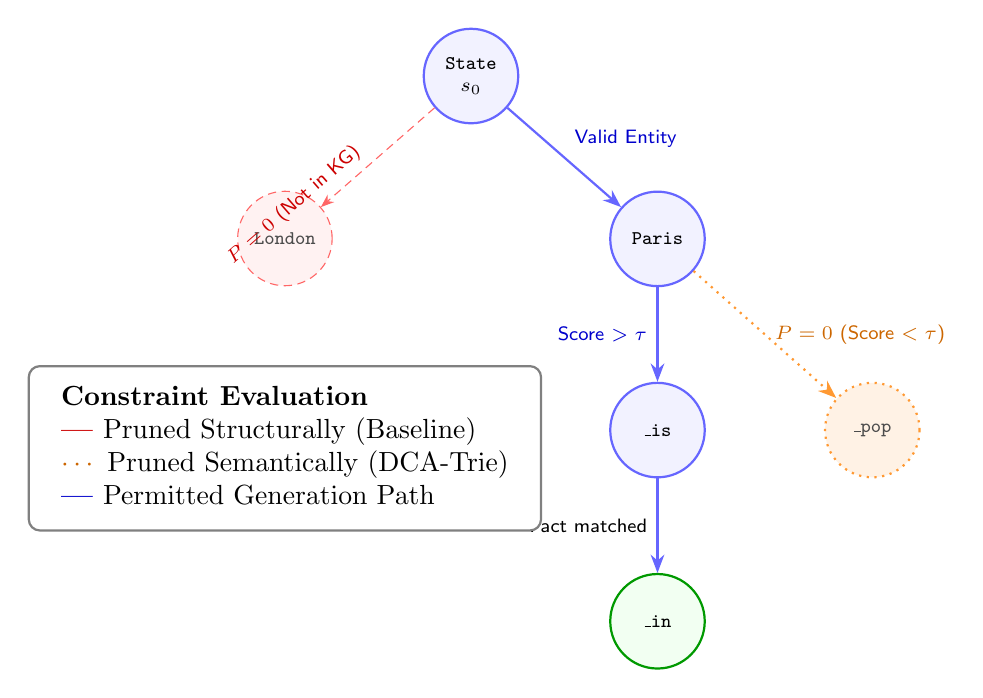
\begin{tikzpicture}[
            node distance=1.2cm and 1.5cm,
            trie/.style={circle, draw=blue!60, fill=blue!5, thick, minimum size=1.2cm, inner sep=1pt, align=center, font=\scriptsize\ttfamily},
            leaf/.style={circle, draw=green!60!black, fill=green!5, thick, minimum size=1.2cm, inner sep=1pt, align=center, font=\scriptsize\ttfamily},
            struct_fail/.style={circle, draw=red!60, fill=red!5, densely dashed, minimum size=1.2cm, inner sep=1pt, text=black!70, align=center, font=\scriptsize\ttfamily},
            sem_fail/.style={circle, draw=orange!80, fill=orange!10, thick, dotted, minimum size=1.2cm, inner sep=1pt, text=black!70, align=center, font=\scriptsize\ttfamily},
            valid_arrow/.style={-{Stealth[scale=1.0]}, thick, draw=blue!60},
            s_fail_arrow/.style={-{Stealth[scale=1.0]}, densely dashed, draw=red!60},
            sem_fail_arrow/.style={-{Stealth[scale=1.0]}, thick, dotted, draw=orange!80}
            ]

            % Root
            \node[trie] (root) {State\\$s_0$};

            % Level 1
            \node[trie, below right=1.2cm and 1.5cm of root] (t1) {Paris};
            \node[struct_fail, below left=1.2cm and 1.5cm of root] (inv1) {London};

            % Level 2 from Paris
            \node[trie, below=1.2cm of t1] (t3) {\_is};
            \node[sem_fail, right=1.5cm of t3] (sem1) {\_pop};

            % Level 3
            \node[leaf, below=1.2cm of t3] (t5) {\_in};

            % Annotations / Edges
            \draw[s_fail_arrow] (root) -- node[above left, sloped, font=\scriptsize\sffamily, text=red!80!black] {$P=0$ (Not in KG)} (inv1);
            \draw[valid_arrow] (root) -- node[above right, font=\scriptsize\sffamily, text=blue!80!black] {Valid Entity} (t1);

            \draw[valid_arrow] (t1) -- node[left, font=\scriptsize\sffamily, text=blue!80!black] {Score $>\tau$} (t3);
            \draw[sem_fail_arrow] (t1) -- node[right, font=\scriptsize\sffamily, text=orange!80!black] {$P=0$ (Score $<\tau$)} (sem1);

            \draw[valid_arrow] (t3) -- node[left, font=\scriptsize\sffamily] {Fact matched} (t5);

            % Legend
            \node[draw=black!50, rounded corners, fill=white, inner sep=0.2cm, thick, anchor=north] at ([yshift=-1cm]inv1.south) {
                \begin{tabular}{l}
                    \textbf{Constraint Evaluation}                                        \\
                    \textcolor{red!80!black}{\textbf{---}} Pruned Structurally (Baseline) \\
                    \textcolor{orange!80!black}{$\cdots$} Pruned Semantically (DCA-Trie)  \\
                    \textcolor{blue!80!black}{\textbf{---}} Permitted Generation Path
                \end{tabular}
            };

        \end{tikzpicture}
    }
    \vspace{0.3cm}
    \caption{Trie-based generation space under DCA-Trie. While static oracles only prune tokens entirely absent from the KG (e.g., ``London''), the dynamic context-aware oracle explicitly sets the probability of structurally valid but contextually irrelevant tokens (e.g., ``\_pop'') to zero before softmax, optimizing search efficiency.}
    \label{fig:kg_trie_search}
\end{figure}

The leading implementation, Graph-Constrained Reasoning (GCR) \citep{luo2025-graph-constrained-reasoning}, constructs a KG-Trie before decoding begins. This trie maps every single structurally valid knowledge graph path within $L$ hops of the question entities over the LLM's token vocabulary. During beam search, GCR ensures that every generated token rigorously follows a permitted trie branch.

\subsection{The Permissiveness Problem}

While GCR successfully blocks structurally invalid tokens, it conflates structural validity with contextual relevance. The GCR oracle calculates the valid token set strictly as a function of the graph $\mathcal{G}$ and the starting entities $\mathcal{E}_q$:
\begin{equation}
    \mathcal{W}_{\text{val}}^{\text{GCR}}(t) = f(\mathcal{G},\, \mathcal{E}_q)
\end{equation}

This static oracle ignores the question itself. In high-degree graphs, a multi-hop query can yield tens of thousands of valid paths. If an oracle admits 8,000 reasoning chains to answer a question that requires a single specific fact, the LLM must still use its parametric memory to guess the correct path among the noise. The oracle has made the generation technically faithful to the graph, but entirely permissive to irrelevant information. This reintroduces the exact hallucination risk constrained decoding was built to avoid \citep{li2024-decoding-on-graphs}.

\section{Methodology}

To resolve the permissiveness problem, we require an oracle that is aware of both the graph structure and the evolving conversational context.

\subsection{Dynamic Context-Aware Trie (DCA-Trie)}

The Dynamic Context-Aware Trie (DCA-Trie) upgrades the constraint oracle to condition on the semantic intent of the query $q$ and the currently generated prefix $y_{<t}$:
\begin{equation}
    \mathcal{W}_{\text{val}}^{\text{DCA}}(t) = f(\mathcal{G},\, \mathcal{E}_q,\, q,\, y_{<t})
\end{equation}

\begin{figure}[htbp]
    \centering
    \resizebox{0.95\textwidth}{!}{
        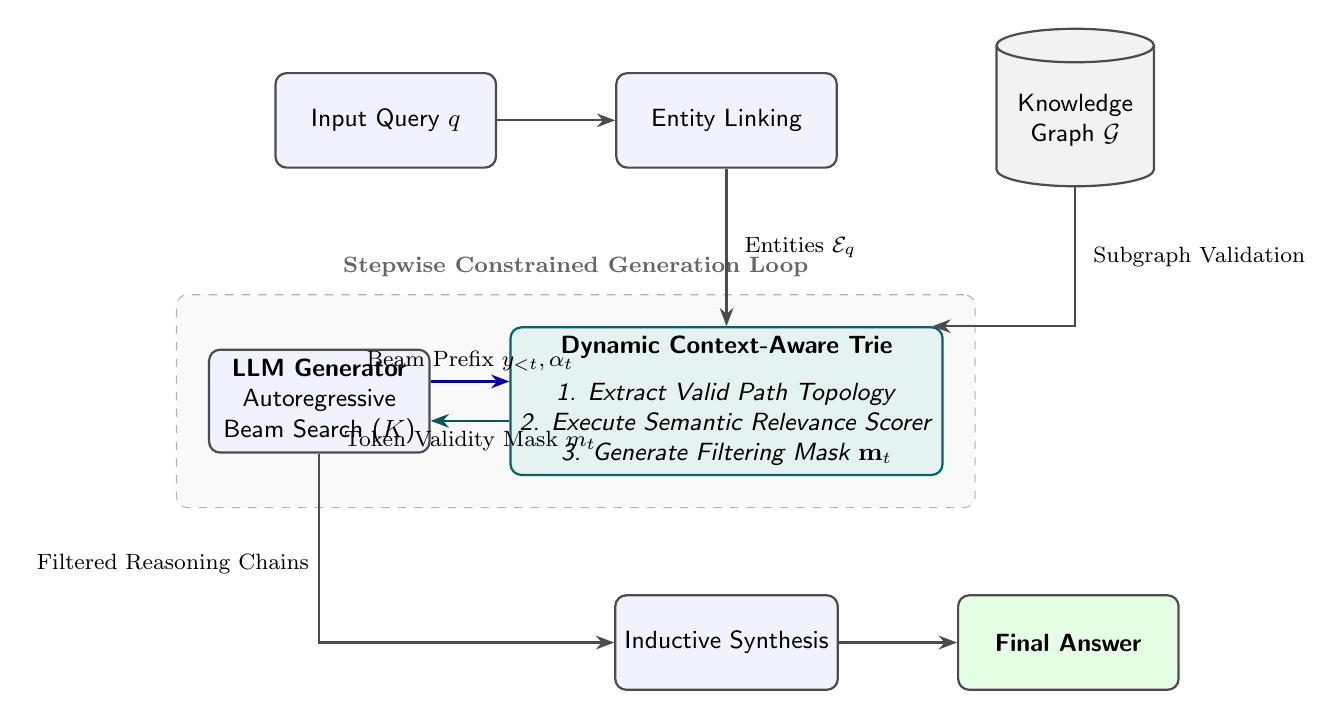
\begin{tikzpicture}[
                >=Stealth,
                node distance=1.5cm,
                font=\small\sffamily,
                block/.style={rectangle, draw=black!70, fill=blue!5, rounded corners, thick, minimum width=2.8cm, minimum height=1.2cm, align=center},
                highlight/.style={rectangle, draw=teal!80!black, fill=teal!10, rounded corners, thick, minimum width=4.5cm, minimum height=1.5cm, align=center},
                db/.style={cylinder, draw=black!70, fill=gray!10, shape border rotate=90, aspect=0.25, thick, minimum width=2cm, minimum height=2cm, align=center},
                arrow/.style={->, thick, draw=black!70},
                group/.style={rectangle, draw=black!30, dashed, inner sep=0.4cm, rounded corners}
            ]

            % Nodes
            \node[block] (query) {Input Query $q$};
            \node[block, right=1.5cm of query] (el) {Entity Linking};

            \node[db, right=2.0cm of el] (kg) {Knowledge\\Graph $\mathcal{G}$};

            \node[highlight, below=2cm of el] (oracle) {\textbf{Dynamic Context-Aware Trie} \\[0.2cm]
                \textit{1. Extract Valid Path Topology} \\ \textit{2. Execute Semantic Relevance Scorer} \\ \textit{3. Generate Filtering Mask $\mathbf{m}_t$}};

            \node[block, fill=blue!5, left=1.0cm of oracle] (llm) {\textbf{LLM Generator} \\ Autoregressive \\ Beam Search ($K$)};

            \node[block, below=1.5cm of oracle] (ir) {Inductive Synthesis};
            \node[block, fill=green!10, right=1.5cm of ir] (ans) {\textbf{Final Answer}};

            % Routing/edges
            \draw[arrow] (query) -- (el);
            \draw[arrow] (el) -- node[right, font=\footnotesize, xshift=0.1cm] {Entities $\mathcal{E}_q$} (oracle);
            \draw[arrow] (kg) |- node[near start, right, font=\footnotesize, xshift=0.1cm] {Subgraph Validation} (oracle.20);

            % Interaction LLM <-> Oracle
            \draw[->, thick, draw=blue!70!black, transform canvas={yshift=0.25cm}] (llm.east) -- node[above, font=\footnotesize, text=black] {Beam Prefix $y_{<t}, \alpha_t$} (oracle.west);
            \draw[<-, thick, draw=teal!70!black, transform canvas={yshift=-0.25cm}] (llm.east) -- node[below, font=\footnotesize, text=black] {Token Validity Mask $m_t$} (oracle.west);

            \draw[arrow] (llm) |- node[near start, left, font=\footnotesize, yshift=-0.2cm] {Filtered Reasoning Chains} (ir);
            \draw[arrow] (ir) -- (ans);

            % Backgrounds
            \begin{scope}[on background layer]
                \node[group, fill=gray!5, fit=(llm)(oracle)] (decoding_group) {};
                \node[above=0.1cm of decoding_group, font=\footnotesize\bfseries, text=black!60] {Stepwise Constrained Generation Loop};
            \end{scope}

        \end{tikzpicture}
    }
    \vspace{0.2cm}
    \caption{The DCA-Trie System Architecture. By sitting between the Knowledge Graph and the LLM, the constraint oracle dynamically filters logits at each beam search step. It combines structural logic (is the path valid?) with semantic relevancy modeling (does the path address $y_{<t}$?), shrinking the autoregressive search space.}
    \label{fig:architecture}
\end{figure}

The architecture injects a semantic relevance scorer directly into the oracle layer, operating ahead of the logit masking step. Given a candidate path $p$, the question $q$, and the partial generation $y_{<t}$, the system encodes both the proposed path and the current context into dense vector embeddings using \texttt{all-MiniLM-L6-v2} \citep{reimers2019sbert}. The semantic relevance score is defined as the cosine similarity between these encodings:

\begin{equation}
    \text{score}(p,\, q,\, y_{<t}) = \cos\!\bigl( E(\text{str}(p)),\, E(\text{query}(q, y_{<t})) \bigr)
\end{equation}

A candidate path prefix is only permitted in the trie if its cosine similarity exceeds a learned threshold $\tau$. This forces every constrained beam to prove both its structural validity (it exists in the graph) and its semantic relevance (it answers the question).

\subsection{The Semantic Irrelevance Ratio (SIR)}

We propose the Semantic Irrelevance Ratio (SIR) to empirically evaluate the efficiency of constraint oracles. Standard metrics like Hits@1 measure if the model eventually found the right answer. They do not measure how much noise the model had to sort through to get there.

SIR explicitly quantifies the redundancy in the oracle's search space. A candidate path $p$ is flagged as irrelevant if its contextual similarity falls below a strict baseline threshold $\tau_{\text{ref}}$ (set independently from the operational threshold $\tau$):
\begin{equation}
    \text{irrelevant}(p, q, y_{<t}) = \mathbf{1}\!\left[
        \cos\!\bigl(E(p),\; E(\text{concat}(q, y_{<t}))\bigr) < \tau_{\text{ref}}
        \right]
\end{equation}

For a given question $q$ at step $t$, the SIR is the proportion of admitted paths $\mathcal{P}(q, t)$ that are irrelevant:
\begin{equation}
    \text{SIR}(q, t) = \frac{\sum_{p \in \mathcal{P}(q,t)} \text{irrelevant}(p, q, y_{<t})}{|\mathcal{P}(q, t)|}
\end{equation}

An SIR approaching $1.0$ indicates search space bloat: the oracle has failed to prune useless paths. An SIR approaching $0.0$ implies a perfectly focused search spanning only highly relevant facts.

\subsection{Design Requirements}

Our DCA-Trie implementation strictly adheres to three methodological constraints:
\begin{enumerate}
    \item \textbf{Structural Faithfulness:} DCA-Trie must maintain 100\% ground-truth structural validity. Every admitted token must exist in the underlying KG.
    \item \textbf{Relevance Reduction:} The corpus-average SIR under DCA-Trie must be significantly lower than under the unmodified GCR oracle.
    \item \textbf{Recall Preservation:} Semantic pruning must not aggressively sever the gold path. The false negative rate (gold path incorrectly pruned) must remain below 5\% on validation splits.
\end{enumerate}

\section{Conclusion}

Knowledge graph-constrained decoding is theoretically necessary to overcome the innate hallucination vulnerabilities of large language models. However, existing static architectures rely entirely on structural graph boundaries, resulting in highly permissive oracles that overwhelm the model with valid but semantically useless paths. The Dynamic Context-Aware Trie (DCA-Trie) bridges this gap by merging structural generation constraints with real-time semantic filtering. By optimizing for the Semantic Irrelevance Ratio (SIR), DCA-Trie tightens the multi-hop search space, allowing LLMs to execute complex reasoning chains efficiently, accurately, and without hallucination.

\bibliographystyle{plainnat}
\bibliography{references}

\end{document}
